\documentclass[12pt]{book}
\usepackage[utf8]{inputenc}
\usepackage[left=25mm,right=25mm,top=15mm,bottom=30mm]{geometry}
\usepackage{amsmath} % math
\usepackage{amssymb} % math
\usepackage{graphicx} % to use \includegraphics{}
\usepackage{diagbox} % to make tables
\usepackage{verbatim} %use comment 주석처리
\usepackage{multirow}
\usepackage[labelformat=simple]{caption}
\usepackage{subcaption}
\usepackage{wrapfig}
\usepackage[hangul]{kotex}
\usepackage{color}
\usepackage[hidelinks]{hyperref}
\usepackage[per-mode=symbol]{siunitx}
\sisetup{inter-unit-product =\cdot} % http://tex.stackexchange.com/questions/59032/how-to-format-si-units
%\graphicspath{{images/}}
%\usepackage{cleveref}
\usepackage{multicol}
\usepackage{array}
\usepackage{gensymb}
\usepackage{siunitx}

\usepackage{fancyhdr}

\pagestyle{fancy}
\fancyhf{}
\rhead{GSHS}
\lhead{circuitikz components}
\cfoot{\thepage}
\newcommand\tab[1][1cm]{\hspace*{#1}}
\renewcommand{\headrulewidth}{2pt}
\renewcommand{\footrulewidth}{1pt}

%\usepackage{draftwatermark}
%\SetWatermarkText{\includegraphics{PNSlogo.png}}

%\renewcommand{\thefootnote}{\fnsymbol{footnote}}

\begin{document}
	\begin{table}[]
		\begin{tabular}{lll}
			component  & node name               & image \\
			접지         & ground                  & 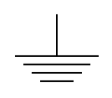
\includegraphics[height=0.045\linewidth]{./images/circuitikz_1.png}       \\
			전류계        & ammeter                 & 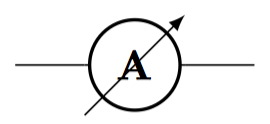
\includegraphics[height=0.045\linewidth]{./images/circuitikz_2.png}       \\
			전압계        & voltmeter               & 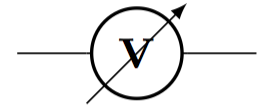
\includegraphics[height=0.045\linewidth]{./images/circuitikz_3.png}        \\
			저항계        & ohmmeter                & 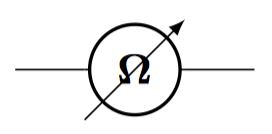
\includegraphics[height=0.045\linewidth]{./images/circuitikz_4.png}       \\
			램프         & lamp                    & 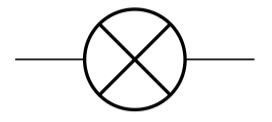
\includegraphics[height=0.045\linewidth]{./images/circuitikz_5.png}        \\
			저항         & R                       & 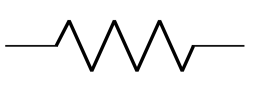
\includegraphics[height=0.045\linewidth]{./images/circuitikz_6.png}        \\
			가변저항       & vR                      & 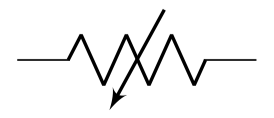
\includegraphics[height=0.045\linewidth]{./images/circuitikz_7.png}       \\
			다이오드       & Do                      & 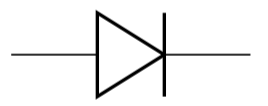
\includegraphics[height=0.045\linewidth]{./images/circuitikz_8.png}       \\
			발광다이오드     & leDo                    & 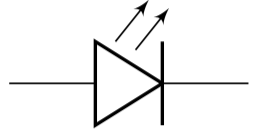
\includegraphics[height=0.045\linewidth]{./images/circuitikz_9.png}       \\
			축전기(커패시터)  & C                       & 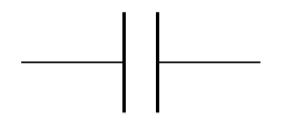
\includegraphics[height=0.045\linewidth]{./images/circuitikz_10.png}       \\
			전해축전기      & pC                      & 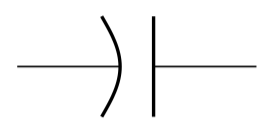
\includegraphics[height=0.045\linewidth]{./images/circuitikz_11.png}       \\
			유도기(인덕터) 1 & L                       & 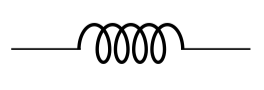
\includegraphics[height=0.045\linewidth]{./images/circuitikz_12.png}       \\
			건전지 1      & battery                 &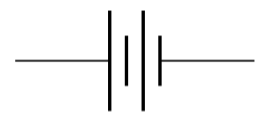
\includegraphics[height=0.045\linewidth]{./images/circuitikz_14.png}       \\
			건전지 2      & battery2                & 
\includegraphics[height=0.045\linewidth]{./images/circuitikz_15.png}       \\
			직류전원장치     & american voltage source & 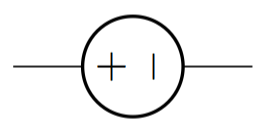
\includegraphics[height=0.045\linewidth]{./images/circuitikz_16.png}       \\
			교류전원장치     & sV                      & 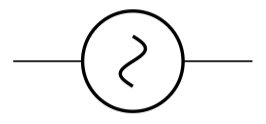
\includegraphics[height=0.045\linewidth]{./images/circuitikz_17.png}       \\
		 	스위치        & nos                     & 
\includegraphics[height=0.045\linewidth]{./images/circuitikz_18.png}       \\
			스위치 &  ncs                       & 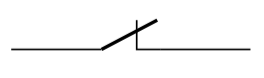
\includegraphics[height=0.045\linewidth]{./images/circuitikz_24.png}       \\
			푸쉬 스위치     & push button             & 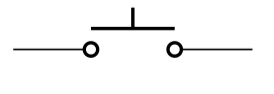
\includegraphics[height=0.045\linewidth]{./images/circuitikz_19.png}       \\
			NPN 트랜지스터  & npn                     &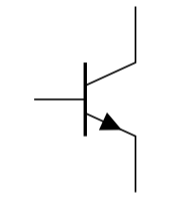
\includegraphics[height=0.045\linewidth]{./images/circuitikz_20.png}        \\
			PNP 트랜지스터  & pnp                     & 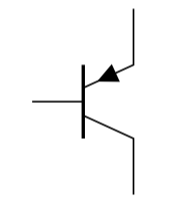
\includegraphics[height=0.045\linewidth]{./images/circuitikz_21.png}       \\
			모터         & elmech                  &  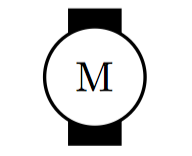
\includegraphics[height=0.045\linewidth]{./images/circuitikz_22.png}      \\
			변압기        & transformer             &   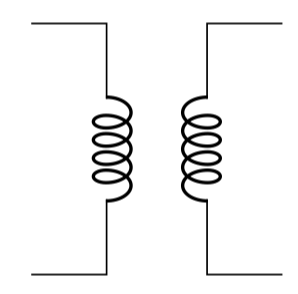
\includegraphics[height=0.045\linewidth]{./images/circuitikz_23.png}    
		\end{tabular}
	\end{table}
	
\end{document}